% !TEX encoding = UTF-8 Unicode
\section{Einleitung}

Weltweit beanspruchen mehr als 4.7 Milliarden Menschen einen mobilen Zugang. Diese Zahl wird bis zum Jahre 2020 auf 5.6 Milliarden anwachsen \cite{gsma2016} und dementsprechend ist der Einfluss der Mobilkommunikation auf die heutige Gesallschaft offensichtlich. Seit dem Jahr 2005 hat sich die Verfügbarkeit von mobiler Kommunikation mehr als verdoppelt und dies resultierte in einer Vielzahl neuer Nutzer und Nutzergruppen \cite{gsma2012}.

\begin{figure}[H]
\centering
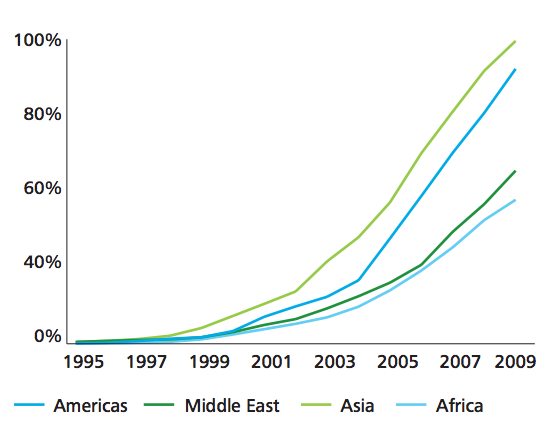
\includegraphics[width=0.5\textwidth]{pictures/mobpen.png}
\caption{Verfügbarkeit der Mobilkommunikation}
\label{fig:mobpen}
\end{figure}

Hinzu kommt der technologische Wandel, der wie die steigende Nutzerzahl einen direkten Einfluss auf ökonomischer Ebene hat. Laut einem Bericht der Global System for Mobile Communications Association (GSMA) hatte zwischen 2008 und 2011 eine 10\% höhere 3G Verfügbarkeit eine Steigerung des Bruttoinlandproduktes (pro Kopf) (BIP) um 0.15 Prozentpunkte zufolge \cite{gsma2012}. Unter 3G wird hier das Mobilfunksystem der dritten Generation verstanden, welches die Anforderungen des International Mobile Communications-2000 Standards (IMT-2000) erfüllte \cite{schiller2003mobile}.   

Mobile Geräte sind in der heutigen Gesellschaft sehr weit verbreitet und weitestgehend akzeptiert. Durch die wachsende Nutzerzahl ist die Netzausweitung und die damit verbundene Verfügbarkeit für Unternehmen äußerst wichtig. Dazu kommt der technologische Wandel und die Notwendigkeit der stetigen Aufrechterhaltung und Erweiterung der Infrastruktur. Für Mobilfunkbetreiber bedeutet dies ein Milliardengeschäft. Aus diesem Grund werden in dieser Seminararbeit zwei Unternehmen aus verschiedenen Gebieten untersucht und miteinander verglichen. Zum einen die \textit{Deutsche Telekom} und zum anderen \textit{China Mobile}. Die Tätigkeitsbereiche mögen zwar sehr ähnlich sein, die Beveölkerungsdichte und die Nutzerzahl sind jedoch sehr verschieden. 

Es wird die Netzausweitung der vierten Generation (4G) aus betriebswirtschaftlicher Sicht betrachtet. Ebenfalls werden die unternehmerischen Erträge miteinander verglichen und es werden in beiden Fällen die Ertragsquellen genannt.

\section{Grundlagen}
Um die Unternehmen \textit{China Mobile} und \textit{Deutsche Telekom} miteinander vergleichen zu können, müssen Grundbegriffe aus Betriebswirtschaftlehre und Mobilkommunikation eingeführt werden. Es folgen Erläuterungen der wichtigsten Begriffe aus beiden Teilbereichen und im Falle der betriebswirtschaftlichen Kennzahlen auch graphische Übersichten. 

\subsection{Begrifflichkeiten der Betriebswirtschaftslehre}
Bis man sich den Kennzahlen widmen kann, muss man definieren was ein Unternehmen ist und was genau ein Unternehmen zu einem wirtschaftlichen Unternehmen macht.

\subsubsection{Unternehmensziele}

Unternehmen versuchen stets wirtschaftlich zu handeln. Dieses Handeln unterliegt dem \textit{ökonomischen Prinzip}, welches sich hauptsächlich mit zwei Aspekten befasst \cite{muller}.

\begin{enumerate}
\item Minimalprinzip: Erreichen eines Ziels mit minimalem Mitteleinsatz oder
\item Maximalprinzip: Maximierung der Zielgröße bei gegebenen Mitteln
\end{enumerate}

Zusätzlich existiert ein drittes Prinzip, das \textit{Allgemeine Extremumprinzip}, welches anstrebt ein möglichst gutes Verhältnis zwischen Aufwand und Ertrag herzustellen. Dieses ist jedoch weniger ein eigenständiges Prinzip sondern vielmehr eine Kombination bzw. ein Kompromiss zwischen  \textit{Minimal-} und \textit{Maximalprinzip}. 

Darüber hinaus muss das \textit{finanzielle Gleichgewicht} eingehalten werden. Dies bedeutet, dass das Unternehmen zu jeder Zeit in der Lage sein muss ihren Zahlungsverpflichtungen nachzugehen \cite{muller}.

Neben \textit{Erfolgszielen}, die sich hauptsächlich an Kenngrößen orientieren, gibt es auch \textit{Sachziele}, die sich davon lösen und andere Bereiche anstreben \cite{domschke}. Diese sind auch für den Bereich der Telekommunikation, mit dem sich diese Ausarbeitung befasst, relevant.

\label{unternehmensziele}
\begin{itemize}
\item \textbf{Leistungsziele:} Ziele bezüglich des Marktes bzw. des Produktes, Produktqualität Marktstellung etc.
\item \textbf{Finanzziele:} Zahlungsfähigkeit des Unternehmens \& Kapitalverfügbarkeit
\item \textbf{Führungsziele:} Ziele im Zusammenhang mit der Unternehmensstruktur, dem Führungsstil 
\item \textbf{Soziale Ziele:} gerechte Entlohnung, günstige Arbeitsbedingungen sowie Sozialleistungen
\item \textbf{Ökologische Ziele:} Ziele Bereich des Umweltschutzes
\end{itemize}

Unternehmerische Erfolge werden oftmals anhand von Kennzahlen festgemacht. Dabei existiert eine Vielzahl von verschiedensten Kennziffern, die auf die Interessen der jeweiligen Personen zugeschnitten sind. So ist beispielsweise \textit{Return on Investment} (ROI) der Quotient aus Gewinn zuzüglich der Fremdkapitalzinsen und eingesetztem Kapital \cite{domschke}. Das Fremdkapital ist hierbei dasjenige Kapital, welches dem Unternehmen von Gläubigern zur Verfügung gestellt worden ist.

\begin{equation}
\frac{\text{(Gewinn durch eingesetztes Kapital - eingesetztes Kapital)}}{\text{eingesetztes Kapital}}
\end{equation}

Die soeben genannte Kennzahl (ROI) besagt wie \glqq erfolgreich\grqq \ eine Kapitalanlage war und ist demnach für (potentielle) Investoren von großem Interesse. Bei einer Investition von $10.000\text{\euro}$ und einem beispielhaften Gewinn von $20.000\text{\euro}$ wäre der ROI $\frac{10.000\text{\euro}}{10.000\text{\euro}}$ oder $100\%$. 

Im Folgenden werden drei Kennzahlen eingeführt, die durchgehend in den Jahresberichten von China Mobile und der Deutschen Telekom gebraucht werden. Diese werden auch später in Abschnitt \ref{sec:vergleich} im direkten Vergleich einander gegenübergestellt.

\subsubsection{Gewinn- und Verlustrechnung}

Bei einem Jahresabschluss eines Unternehmens, also bei einem rechnerischen Abschluss eines Geschäftsjahres, werden Kenngrößen aufgezählt und gegenüber gestellt. Neben einer Bilanz wird auch die Gewinn- und Verlustrechnung aufgeführt, die die unternehmerischen Einnahmen und Ausgaben aufzeigt. Unter der Bilanz versteht man eine Gegenüberstellung von \textit{Passiva}, also dem Ursprung der unternehmerischen Mittel und \textit{Aktiva}, welche Auskunft darüber geben für welche Zwecke diese Mittel eingesetzt worden sind \cite{muller}. 

Das Hauptaugenmerk wird hier jedoch bei der Gewinn- und Verlustrechnung und der darauf anknüpfenden finanzwirtschaftlichen Analayse liegen, da die Bilanz nur wenig Information für den Unternehmensvergleich bietet. Bei einer Gewinn- und Verlustrechnung werden die Aufwendungen den Erträgen gegenübergestellt. Im Vergleich zur Bilanz sind diese sehr detailliert, da die Bilanz lediglich die Höhe des Gewinnes/des Verlustes zeigt und nicht die tatsächlichen Aufwendungen \cite{muller}. Eine beispielhafte Rechnung ist der folgenden Grafik zu entnehmen:


\begin{figure}[H]
\centering
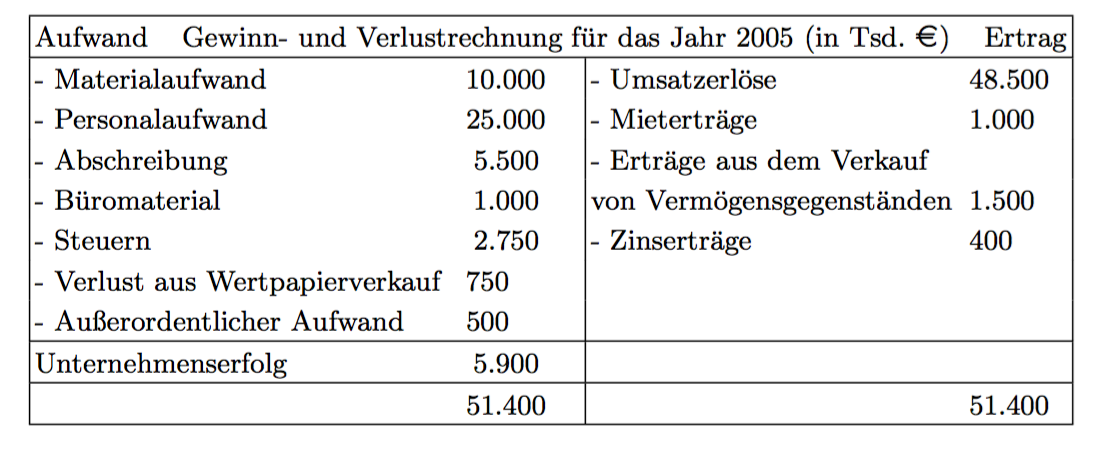
\includegraphics[width=0.75\textwidth]{pictures/guv.png}
\caption{Beispielhafte Gewinn- und Verlustrechnung}
\label{fig:guv}
\end{figure}

\subsubsection{Finanzwirtschaftliche Analyse}

Es folgt eine Definition einiger wichtiger Kenngrößen, die Informationen über das Wirtschaften von Unternehmen bieten sollen. 

\textit{Earnings Before Interest and Taxes} (EBIT) ist eine Kenngröße, die Auskunft über den Gewinn eines Unternehmens bieten soll. Hierbei werden die Zinsen und Steuern nicht betrachtet, sodass EBIT sich sehr gut für einen Unternehmensvergleich eignet. Neben EBIT existiert eine erweiterte Kenngröße, die zusätlich noch den Gewinn ohne Abschreibungen auf Sachanlagen und immaterielle Vermögensgegenstände betrachtet \cite{bwlformeln}.

\begin{enumerate}
\item \textbf{EBIT} = Jahresabschluss + Steueraufwand - Steuererträge + Zinsaufwand - Zinsertrag
\item \textbf{EBITDA} = EBIT + Abschreibungen auf das Anlagevermögen - Zuschreibungen zum Anlagevermögen 
\end{enumerate}  

Eine weitere Kennzahl ist der \textit{Cash-Flow}. Dieser spiegelt die Fähigkeit eines Unternehmens das Fremdkapital zurückzuzahlen. Der sogenannte \textit{Cash-Flow} soll dabei komplett zur Schuldungstilgung verwendet werden. In der folgenden Formel wird der Überschuss der Erträge über die Aufwendungen dargestellt.

\begin{enumerate}
\item \textbf{Cash-Flow} = Gewinn + Abschreibung + Erhöhung der Rückstellungen 
\end{enumerate}

Der Cash-Flow ist ebenfalls ein Indikator für die finanzielle Autonomie des Unternehmens, da durch ihn indirekt die Unabhängigkeit vom Fremdkapital dargstellt wird \cite{muller}.

Als letzte Kenngröße wird die \textit{Liquidität} eingeführt. Ein Unternehmen ist liquide, wenn es zu jedem Zeitpunkt den Verbindlichkeiten nachkommen kann \cite{muller}. Bei dem Vergleich zwischen der \textit{Deutschen Telekom} und \textit{China Mobile} wird insbesondere auf Risiken im Bezug auf den Liquiditätsverlust eingegangen. Die folgende Abbildung zeigt die drei Liquiditätsstufen.

\begin{figure}[H]
\centering
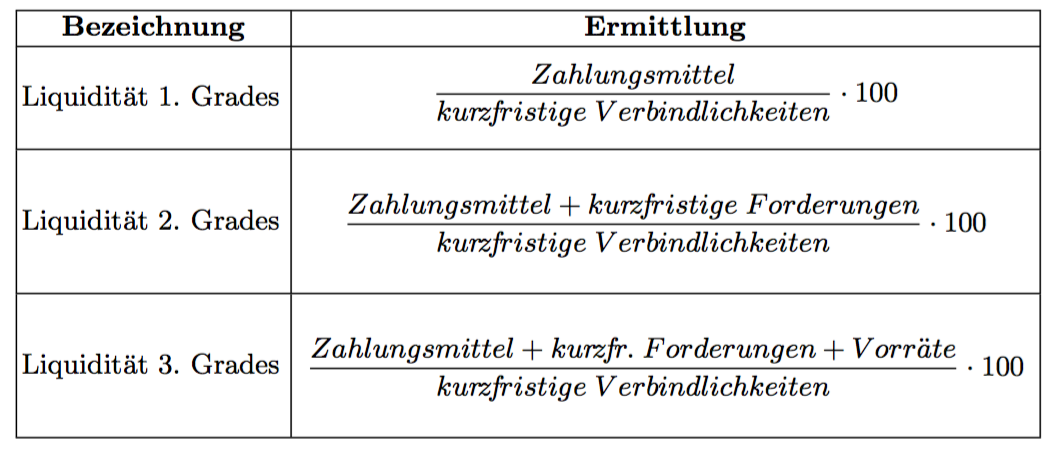
\includegraphics[width=0.85\textwidth]{pictures/liquidity.png}
\caption{Liquiditätsstufen}
\label{fig:liquidity}
\end{figure}

\subsection{Mobilkommunikation}

Die beiden vorgestellten Unternehmen verwenden Begrifflichkeiten und Technologien, die nicht unbedingt offensichtlich sind. Es folgt ein kurzer Überblick. 

\subsubsection{4G}

Unter 4G versteht man ein Mobilfunksystems vierten Generation, welches die Anforderungen des IMT Advanced Standards von 2008 umsetzen soll. \textit{Long-Term Evolution} (LTE) wurde im Jahre 2009 zum ersten Mal kommerziell verwendet und wird seitdem ständig vom Third Generation Partnership Project (3GPP) weiterentwickelt \cite{lte}. Ein direkter Vergleich zwischen 3G und 4G würde hier den Rahmen sprengen und aus diesem Grund werden nur die vermeintlich auffälligsten Verbesserungen genannt. Die zuvor verbreiteten 4G Kampagnen sind in Wahrheit kein wahres Mobilfunksystem der vierten Generation, da sie nur teilweise die Anforderungen des IMT Standards erfüllen.

Die folgende tabellarische Darstellung zeigt den Unterschied zwischen \glqq 3.9G\grqq \ und 4G.

\begin{figure}[H]
\centering
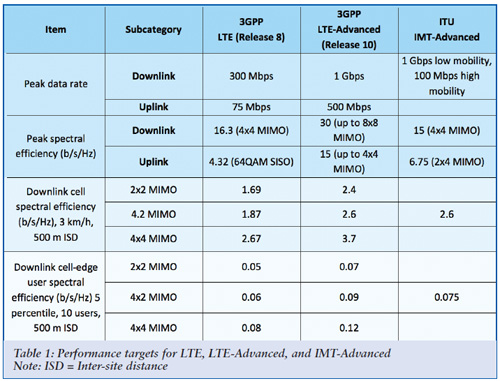
\includegraphics[width=0.9\textwidth]{pictures/lteadv.jpg}
\caption{Vergleich zwischen LTE und LTE+ \cite{ltevergleich}}
\label{fig:lteplus}
\end{figure}

Bei 3G befand man sich im Mbit/s Bereich, bei echtem 4G ist man hingegen im Gbit/s Bereich. Ebenfalls wird die Quality-of-Service durch die erhöhten Datenraten verbessert, da die spektrale Effizienz sich ebenfalls erhöht hat. Die spektrale Effizienz sagt dabei aus wie effizient Daten auf einer gewissen Bandbreite übertragen werden, d.h. wie effizient das Übertragungsmedium genutzt werden kann \cite{ltevergleich}.   

4G Technologien sind bei beiden Unternehmen von großer Prioriät und wurden im Jahre 2016 weiter aufgebaut und erweitert.

\subsubsection{Internet of Things}

Investitionen und Ausweitungen auf den Bereich des \textit{Internet of Things} (IoT) ist ebenfalls bei beiden Unternehmen zu beobachten. Unter IoT versteht man die Vernetzung von physischen Objekten. Es ermöglicht also beliebige vernetzte Objekte zu kontrollieren und miteinander kommunizieren zu lassen. Es ist gewissermaßen als eine Einbettung der physischen Objekte in einem Netwerk zu sehen \cite{iotcisco}. Sensoren, Heizungsanlagen oder auch Heimautomatisierungssysteme, durch hohe Übertragungsraten und erhöhte Verfügbarkeit der vierten Mobilfunkgeneration lassen sich die Geräte einfacher und effizienter miteinader verknüpfen. Ebenfalls sinkt die Stromversorgung unter LTE Advanced deutlich und dies ist für IoT Geräte sehr vorteilhaft, da diese sehr begrenzte Kapazitäten haben \cite{iotnokia}.  

\subsubsection{Internet Plus}

Als letzten Begriff wird \textit{Internet Plus} eingeführt. Dieser wurde von der chinesischen Regierung eingeführt und beschreibt die Einbindung des Internets in konventiellen Bereichen und Industrien \cite{internetplus}. Das Primärziel der chinesischen Regierung ist dabei eine rapide Steigerung des BIP. Diese Etablierung des Internets und Vernetzung der Industrien soll dabei im Jahre 2018 eine der treibenden Kräfte sein.  

\section{China Mobile}
\label{sec:china}
\subsection{Eckdacten}

China Mobile wurde am 3. September im Jahre 1997 in Hong Kong gegründet und ist heute der führende Mobilfunkanbieter/-betreiber auf dem chinesischen Festland. Das Unternehmen hatte Ende des Jahres 2016 (31.12.2016) 460,647 Angestellte \cite{chinasite}.

Die Kennzahlen und Informationen, die in den folgenden Abschnitten verwendet werden, wurden im März 2017 im Jahresbericht 2016 veröffentlicht \cite{chinareport}. 

Zu Beginn werden die wichtigsten Eckdaten genannt, welche das Wachstum zwischen den Jahren 2015 und 2016 demonstrieren sollen. 

\begin{figure}[H]
\centering
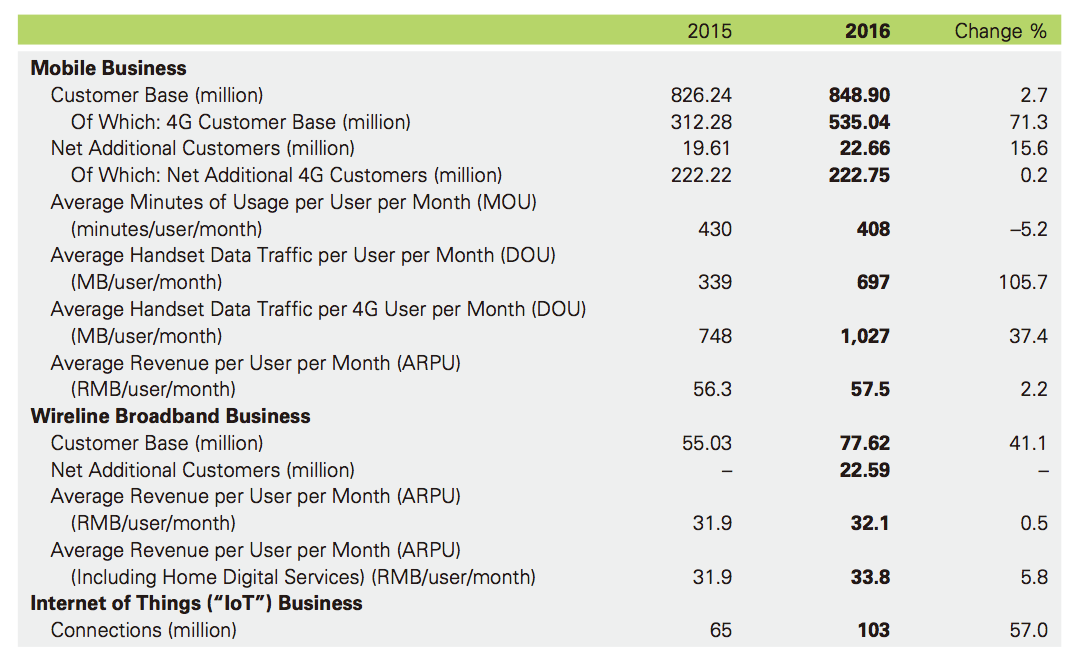
\includegraphics[width=0.85\textwidth]{pictures/china_users}
\caption{Eckdaten}
\label{fig:lteplus}
\end{figure}

Die Nutzerzahl ist von 826 Millionen auf 848 Millionen gestiegen, was einen Zuwachs von $7\%$ bedeutet. Hierbei sei zu vermerken, dass der Nutzeranstieg mit der Zeit aufgrund der Sättigung immer schwieriger wird. Viel interessanter und aussagekräftiger ist hingegen die Anzahl der Kundschaft, die die vierte Generation des Mobilfunknetzes nutzen. Die Nutzeranzahl ist hier drastisch um $71.3\%$ gestiegen was bereits auf die Bestrebungen des Unternehmens deutet. Ebenfalls ist der Datenverbrauch um $105\%$ angestiegen und beim 4G Datenverbrauch ist ebenfalls ein $30\%$-iger Anstieg zu sehen.

Das Hindeuten auf die Bestrebungen bei der 4G Technologie wird in späteren Teilen des Jahresberichts bestätigt. So errichtete China Mobile im Jahre 2016 400.000 4G Basisstationen und brachte somit die Gesamtzahl auf 1.51 Millionen. Bei einer Bevölkerung von 1.37 Milliarden (Stand 2015) sorgte China Mobile für eine flächendeckende Verfügbarkeit für bis zu 1.3 Milliarden Nutzer. 

Zusätzlich zu Neukunden wurde dafür gesorgt, dass 2G/3G Kunden auf die neue Technologie migriert wurden. Dies sorgte dafür, dass das durchschnittliche 4G Datenvolumen pro Kunden das 7.5-fache des Datenvolumens für ältere Generationen betrug.

Neben des herkömmlichen Mobilfunkes wurde das weltweit größte Netzwerk für IoT Geräte errichtet mit mehr als 100 Millionen vernetzten Geräten. 

\subsection{Kennzahlen}

Die soeben genannten Bestrebungen resultierten in einem erhöhten Betriebsergebnis im Vergleich zum Jahre 2015.

\begin{figure}[H]
\centering
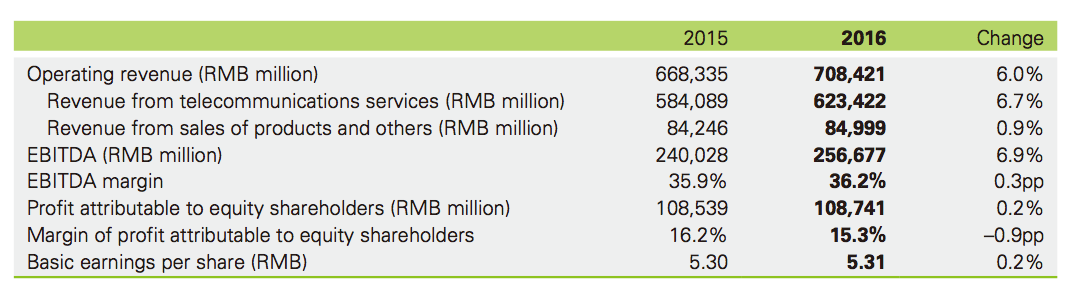
\includegraphics[width=0.85\textwidth]{pictures/finances}
\caption{Finanzielle Analyse von China Mobile}
\label{fig:lteplus}
\end{figure}

Das Betriebsergebnis stieg von 668 Milliarden CNY ($\sim 87.5$ Milliarden \euro) auf 708 Milliarden ($\sim 104.56$ Milliarden \euro). Der EBITDA stieg um $6.9\%$ auf $\sim 33$ Milliarden \euro \ und die Marge, also der Quotient aus EBITDA und Umsatz, betrug $36.2\%$. Die Marge stellt somit das Verhältnis zwischen dem Ertrag und dem Umsatz her. Neben dieser Kennzahlen ist auch interessant durch welche Dienste der Umsatz generiert wurde. 

Der generierte Umsatz durch Anrufe sank um $19.8\%$ auf 210 Milliarden CNY ($\sim 27.5$ Milliarden \euro) und der mobile Datenverbrauch stieg um $30.2\%$ auf 394 Milliarden CNY ($\sim 51.6$ Milliarden \euro). Diese Veränderung sagt viel über die Strategie des Unternehmens aus. Nach und nach werden Kunden Flatrates angeboten und immer mehr Anrufe werden mittels IP-Telefonie getätigt. Selbiges gilt für das Versenden von Nachrichten.  

Beim Cash-Flow sind ebenfalls signifikante Veränderungen zu verzeichnen. So verringerten sich die Aufwendungen um $43.4\%$ auf $48.95$ Milliaden CNY ($\sim 6.4$ Milliarden \euro) und dies deutet auf die erhöhte finanzielle Unabhängigkeit des Unternehmens vom Fremdkapital hin.

\begin{figure}[H]
\centering
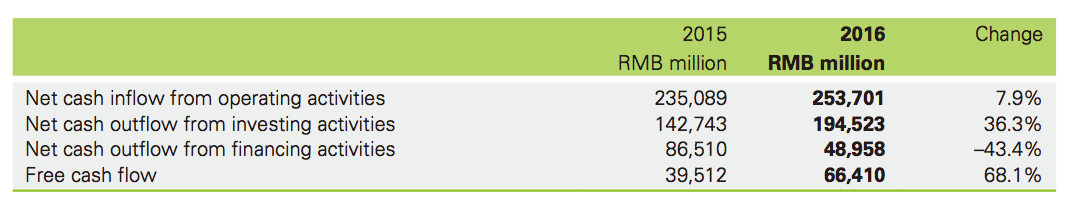
\includegraphics[width=0.85\textwidth]{pictures/cashflow}
\caption{Cash-Flow-Analyse von China Mobile}
\label{fig:lteplus}
\end{figure}

Als letzten Punkt ist noch die Absicherung der unternehmerischen Liquidität zu nennen. China Mobile verfügt, wie auch andere Unternehmen, über Reserven, die bei Bedarf eingesetzt werden können. Bis zu 443 Milliarden CNY ($\sim 58$ Milliarden \euro) können innerhalb eines Jahres beschaffen werden, um im Falle einer vorübergehenden Zahlungsunfähigkeit offenen Zahlungen nachzugehen. 

\section{Deutsche Telekom}

Die Deutsche Telekom AG wurde am 1. Januar 1995 gegründet und ist heute einer der führenden Mobilfunkanbieter/-betreiber in Deutschland und einer der einflussreichsten Anbieter in Europa. Das Unternehmen hatte im Jahr 2016 221,000 Angestellte \cite{telekomsite}.

Die Kennzahlen und Informationen, die in den folgenden Abschnitten verwendet werden, wurden am Anfang des Jahres 2017 veröffentlicht \cite{telekomreport}. 

Zu Beginn werden die wichtigsten Eckdaten, ähnlich China Mobile, genannt. Diese sollen einen Überblick bieten und das Wachstum zwischen den Jahren 2015 und 2016 demonstrieren. 

\subsection{Eckdaten}

Die Telekom verzeichnete im Jahr 2016 einen Nutzerzuwachs von $5.5\%$, von $156.4$ Million zu $165$ Millionen Nutzern. Zum Ende des Kalenderjahres 2016 deckte die Telekom in teilnehmenden Ländern $84\%$ ihrer Kundschaft mit einem 4G Mobilfunknetz ab. Es wird auch durchgehend von einem erhöhten Kundeninteresse bezüglich des 4G Netzes gesprochen, welches durch den Kauf von vielen Smartphones bestätigt wird \cite{telekomreport}.


\begin{figure}[H]
\centering
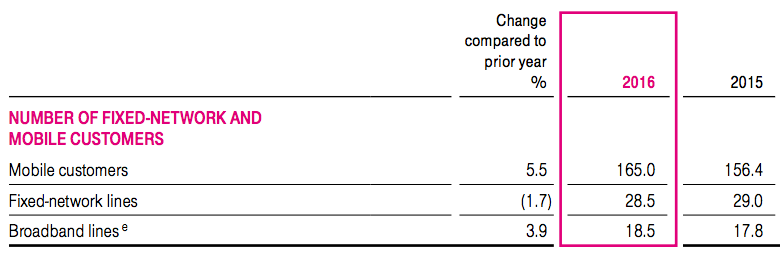
\includegraphics[width=0.85\textwidth]{pictures/telekom_nutzer.png}
\caption{Nutzerzahlen der Telekom}
\label{fig:telekom}
\end{figure}

Eines der Ziele der Telekom ist es bis zum Jahre 2018 eine Abdeckung in teilnehmenden Ländern zwischen $75$ und $95\%$ zu erreichen. Speziell in Deutschland LTE Abdeckung von $95\%$ das Ziel. Wie in Abbildung \ref{fig:telekom} zu sehen, wurde die Zahl der Breitbandleitungen um 700,000 erhöht was wiederum auf die Ausweitung des Mobilfunknetzes der vierten Generation hindeutet. 

Neben der 4G Ausweitung errichtete die Telekom ein System für die Vernetzung von Endgeräten im IoT Bereich mittels Schmalbandkommunikation.   

\subsection{Kennzahlen}

Wie die Abbildung \ref{fig:telekom_gewinn} zeigt, verzeichnete die Telekom ein gestiegenes Betriebsergebnis im Jahre 2016.

\begin{figure}[H]
\centering
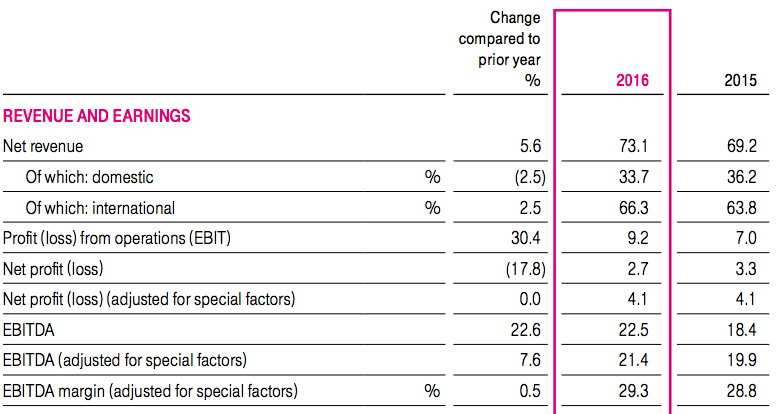
\includegraphics[width=0.85\textwidth]{pictures/telekom_gewinn.png}
\caption{Kennzahlen der Telekom}
\label{fig:telekom_gewinn}
\end{figure}

Die Erträge stiegen um $5.6\%$ auf $73.1$ Milliarden \euro. Die Anteile beim Ertrag innerhalb Deutschlands und außerhalb veränderten sich jedoch. So machten die Gewinne in Deutschland nur noch $33.7\%$ des Gesamtgewinnes aus, was ein absolutes Tief im Vergleich zu den letzten Jahren darstellt.

Der EBITDA stieg um $22.6\%$ auf $22.5$ Milliarden \euro \ und die Marge Betrug $29.3\%$. 

Die Telekom investierte $11$ Milliarden Euro unter anderem auch für die Ausweitung des LTE-Netzes um den Kundenbedürfnissen gerecht zu werden. Diese verwendeten immer weniger die traditionellen Möglichkeiten der mobilen Kommunikation und wichen auf IP-basierte Nachrichtendienste wie WhatsApp oder Facebook aus.

Der Cash-Flow stieg um $9\%$ auf $4.9$ Milliarden \euro. Es wird ein Anwachsen auf bis zu $5.5$ Milliarden \euro \ im Jahre 2017 erwartet. 

Im Falle einer vorübergehenden Zahlungsunfähigkeit verfügt die Telekom über Reserven, die notfalls für $24$ Monate ausreichen und damit die Liquidität auf einem absehbaren Zeitraum garantieren.    

\section{Vergleich}
\label{sec:vergleich}

Beide Unternehmen verzeichneten einen Anstieg im Bezug auf das Betriebsergebnis im Vergleich zum Vorjahr. Bei China Mobile war es ein Anstieg von $6\%$ und der Telekom von $5.6\%$. Die Telekom gewann prozentual mehr Nutzer als China Mobile, $5.5\%$ zu $2.7\%$, aber wie in Abschnitt \ref{sec:china} bereits erwähnt, ist das Wachstum bei einer gewissen Sättigung sehr schwer. Im Falle der Telekom gibt es noch Kundschaft in angrenzenden Ländern.

Sowohl die Telekom als auch China Mobile bemerkten eine deutliche Zunahme im mobilen Datenverbrauch und einen gleichzeitigen Rückgang bei den traditionellen Formen der mobilen Kommunikation. Beides deutet darauf hin, dass viele Nutzer heutzutage zu den IP-basierten, kostenfreien Alternativen greifen.

Die Erträge lassen sich aufgrund der sehr unterschiedlichen Nutzerzahlen nur schwer vergleichen, die EBITDA-Marge hingegen ist ähnlich, $29.3\%$ bei der Telekom und $36.2\%$ bei China Mobile. 

Die Zahlungsfähigkeit ist ebenfalls bei beiden Unternehmen auf einen absehbaren Zeitraum gesichert.  

Insgesamt lässt sich sagen, dass beide Unternehmen, trotz verschiedener Nutzerbasen und Lagen, ähnliche Nutzerverhalten beobachten und ihre Unternehmenspolitik dementsprechend anpassen. Die Jahresberichte unterscheiden sich jedoch grundlegend. China Mobile präsentiert genauere Kennzahlen und bietet mehr Information über das Kundenverhalten an. So wird beispielsweise die direkte Nutzerzahl von 4G Anwendern genannt, was beim Jahresbericht der Telekom nicht der Fall ist. Ebenfalls erkennt man die Bestrebungen des chinesischen Unternehmens und die Gründe für eine Ausweitung des 4G Netzes deutlich klarer.  

\section{Ausblick}

In beiden Fällen lassen sich auch ähnliche Pläne für die Zukunft beobachten. Im Falle von China Mobile ist es Internet Plus, welches für das Vernetzen in verschiedenen industriellen und sozialen Bereichen sorgen soll. Die Telekom plant in der Zukunft eine Ausweitung auf Industrie 4.0 und IoT, was dem Vorhaben von China Mobile weitestgehend entspricht. 

Selbstverständlich sind beide Unternehmen weiterhin an der Ausweitung und Erweiterung des eigenen Netzes interessiert sowie am potentiellen Ausbau ihrer Infrastruktur für weitere Generationen von Mobilfunknetzen.  

\medskip

\bibliographystyle{unsrt}
\bibliography{bib}
